\documentclass[pdftex,english,a4paper,10pt]{infocom}
\usepackage[pdftex,bookmarksnumbered,colorlinks,backref, bookmarks, breaklinks, linktocpage]{hyperref}
\usepackage[pdftex]{graphicx}
\usepackage{isolatin1}
\usepackage{fancyvrb}
\pdfcompresslevel=9
\title{DocBook Demystification HOWTO}
\author{Eric Raymond}
\begin{document}

\maketitle

% --------------------------------------------
% Abstract 
% --------------------------------------------
\begin{abstract}


  This HOWTO attempts to clear the fog and mystery surrounding the
  DocBook markup system and the tools that go with it.  It is aimed at
  authors of technical documentation for open-source projects hosted
  on Linux, but should be useful for people composing other kinds on
  other Unixes as well.  
  
\end{abstract}


% ------------------------   
% Section 
\section{Introduction}
\label{intro}\hypertarget{intro}{}%

A great many major open-source projects are converging on
DocBook as a standard format for their documentation --- projects
including the Linux kernel, GNOME, KDE, Samba, and the Linux
Documentation Project.  The advocates of XML-based "structural markup"
(as opposed to the older style of "presentation markup" exemplified by
troff, Tex, and Texinfo) seem to have won the theoretical
battle.

Nevertheless, a lot of confusion surrounds DocBook and the
programs that support it.  Its devotees speak an argot that is dense
and forbidding even by computer-science standards, slinging around
acronyms that have no obvious relationship to the things you need to
do to write markup and make HTML or Postscript from it.  XML standards
and technical papers are notoriously obscure.  Most DocBook-related
tools are very poorly documented, and their documentation is
especially prone to assume way too much prior knowledge on the
reader's part.

This HOWTO will attempt to clear up the major mysteries
surrounding DocBook and its application to open-source documentation
--- both the technical and political ones.  Our objective is to equip
you to understand not just what you need to do to make documents, but
why the process is as complex as it is --- and how it can be
expected to change as newer DocBook-related tools become
available.

% ------------------------   
% Section 
\section{Why care about DocBook at all?}
\label{id2718555}\hypertarget{id2718555}{}%

There are two possibilities that make DocBook really
interesting.  One is {\em multi-mode rendering} and the
other is {\em searchable documentation
databases}.

Multi-mode rendering is the easier, nearer-term possibility; it's
the ability to write a document in a single master format that can be
rendered in many different display modes (in particular, as both HTML
for on-line viewing and as Postscript for high-quality printed
output).  This capability is pretty well implemented now.

{\em Searchable documentation databases} is
shorthand for the possibility that DocBook might help get us to a
world in which all the documentation on your open-source operating
system is one rich, searchable, cross-indexed and hyperlinked
database (rather than being scattered across several different formats
in multiple locations as it is now).

Ideally, whenever you install a software package on your machine 
it would register its DocBook documentation into your system's
catalog.  HTML, properly indexed and cross-linked to the HTML in the 
rest of your catalog, would be generated.  The new package's
documentation would then be available through your browser.  All
your documentation would would be searchable through an interface
resembling a good Web search engine.

HTML itself is not quite rich enough a format to get us to that
world.  To name just one lack, you can't explicitly declare index
entries in HTML.  DocBook {\em does} have the semantic
richness to support structured documentation databases.  Fundamentally
that's why so many projects are adopting it.

DocBook has the vices that go with its virtues.  Some people
find it unpleasantly heavyweight, and too verbose to be really
comfortable as a composition format.  That's OK; as long as the markup
tools they like (things like Perl POD or GNU Texinfo) can generate
DocBook out their back ends, we can all still get we want.  It doesn't
matter whether or not everybody writes in DocBook --- as long as
it becomes the common document interchange format that everyone uses,
we'll still get unified searchable documentation databases.

% ------------------------   
% Section 
\section{Structural markup: a primer}
\label{id2767054}\hypertarget{id2767054}{}%

Older formatting languages like Tex, Texinfo, and Troff
supported {\em presentation
markup}\index{presentation markup}.  In these systems, the instructions you
gave were about the appearance and physical layout of the text (font
changes, indentation changes, that sort of thing).

Presentation markup was adequate as long as your objective was
to print to a single medium or type of display device.  You run into
its limits, however, when you want to mark up a document so that (a)
it can be formatted for very different display media (such as printing
vs. Web display), or (b) you want to support searching and indexing the
document by its logical structure (as you are likely to want to do,
for example, if you are incorporating it into a hypertext system).

To support these capabilities properly, you need a system of
{\em structural markup}\index{structural markup}.  In structural markup, you describe not
the physical appearance of the document but the logical properties of
its parts.

As an example: In a presentation-markup language, if you want to
emphasize a word, you might instruct the formatter to set it in
boldface.  In
troff(1)
this would look like so:

\begin{Verbatim}[]

All your base
.B are
belong to us!

\end{Verbatim}

In a structural-markup language, you would tell the formatter to
emphasize the word:

\begin{Verbatim}[]

All your base <emphasis>are</emphasis> belong to us!

\end{Verbatim}

 The "\textless{}emphasis\textgreater{}" and \textless{}/emphasis\textgreater{}in the line above
are called {\em markup
tags}\index{markup tags},
or just {\em tags} for short.  They are the
instructions to your formatter.

In a structural-markup language, the physical appearance of the
final document would be controlled by a {\em stylesheet}
\index{stylesheet}.  It is the
stylesheet that would tell the formatter "render emphasis as a font
change to boldface".  One advantage of presentation-markup languages
is that by changing a stylesheet you can globally change the
presentation of the document (to use different fonts, for example)
without having to hack all the the individual instances of (say)
.B in the document itself.

% ------------------------   
% Section 
\section{Document Type Definitions}
\label{id2716782}\hypertarget{id2716782}{}%

(Note: to keep the explanation simple, most of this
section is going to tell some lies, mainly by omitting a lot of 
history.  Truthfulness will be fully restored in a following
section.)

DocBook is a structural-level markup language.  Specifically, it
is a dialect of XML.  A DocBook document is a hunk of XML that uses
XML tags for structural markup.

In order for a document formatter to apply a stylesheet to your
document and make it look good, it needs to know things about the
overall structure of your document.  For example, it needs to know
that a book manuscript normally consists of front matter, a sequence
of chapters, and back matter in order to physically format chapter
headers properly.  In order for it to know this sort of thing, you
need to give it a {\em Document Type
Definition}\index{Document Type Definition!DTD} or DTD. The
DTD tells your formatter what sorts of elements can be in the document
structure, and in what orders they can appear.

What we mean by calling DocBook an `application' of XML is
actually that DocBook is a DTD --- a rather large DTD, with
somewhere around 400 tags in it.

Lurking behind DocBook is a kind of program called a
{\em validating parser}\index{validating parser}.When you format a DocBook document, the
first step is to pass it through a validating parser (the front end of
the DocBook formatter).  This program checks your document against the
DocBook DTD to make sure you aren't breaking any of the DTD's
structural rules (otherwise the back end of the formatter, the part
that applies your style sheet, might become quite confused)

The validating parser will either bomb out, giving you error
messages about places where the document structure is broken, or translate
the document into a stream of {\em formatting events}
which the parser back end combines with the information in your stylesheet
to produce formatted output

Here is a diagram of the whole process:
{{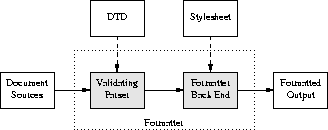
\includegraphics[]{figure1.png}}}

The part of the diagram inside the dotted box is your formatting
software, or {\em toolchain}. Besides the obvious and
visible input to the formatter (the document source) you'll need to
keep the two `hidden' inputs of the formatter (DTD and stylesheet) in
mind to understand what follows.

% ------------------------   
% Section 
\section{Other DTDs}
\label{id2719220}\hypertarget{id2719220}{}%

A brief digression into other DTDs may help make clear what parts of
the previous section were specific to DocBook and what parts are general to
all structural-markup languages.

\href{http://www.tei-c.org/}{TEI} (Text Encoding
Initiative) is a large, elaborate DTD used primarily in academia for
computer transcription of literary texts.  TEI's Unix-based toolchains
use many of the same tools that are involved with DocBook, but with
different stylesheets and (of course) a different DTD.

XHTML, the latest version of HTML, is also an XML application
described by a DTD, which explains the family resemblance between
XHTML and DocBook tags. The XHTML toolchain consists of web browsers
and a number of ad-hoc HTML-to-print utilities.

Many other XML DTDs are maintained to help people exchange
structured information in fields as diverse as bioinformatics and
banking.  You can look at a \href{http://www.xml.com/pub/rg/DTD_Repositories}{ list of
repositories} to get some idea of the variety out
there.

% ------------------------   
% Section 
\section{The DocBook toolchain}
\label{id2719272}\hypertarget{id2719272}{}%

Normally, what you'll do to make XHTML from your
DocBook sources will look like this:

\begin{Verbatim}[]

bash$ xmlto xhtml foo.xml
Convert to XHTML
bash$ ls *.html
ar01s02.html ar01s03.html ar01s04.html index.html

\end{Verbatim}

In this example, you converted an XML-Docbook  document named 
{\tt{foo.xml}} with three top-level sections into an
index page and two parts.  Making one big page is just as easy:

\begin{Verbatim}[]

bash$ xmlto xhtml-nochunks foo.xml
Convert to XHTML
bash$ ls *.html
foo.html

\end{Verbatim}

Finally, here is how you make Postscript for printing:

\begin{Verbatim}[]

bash$ xmlto ps foo.xml       # To make Postscript
Convert to XSL-FO
Making portrait pages on A4 paper (210mmx297mm)
Post-process XSL-FO to DVI
Post-process DVI to PS
bash$ ls *.ps
foo.ps

\end{Verbatim}

To turn your documents into HTML or Postscript, you need an
engine that can apply the combination of DocBook DTD and 
a suitable stylesheet to your document.  Here is how the 
open-source tools for doing this fit together:
{{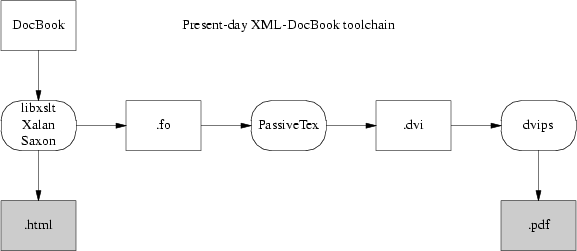
\includegraphics[]{figure2.png}}}

Parsing your document and applying the stylesheet transformation
will be handled by one of three programs.  The most likely one is
xsltproc\index{xsltproc},
the parser that ships with Red Hat 7.3.  The other possibilities are
two Java programs,
Saxon\index{Saxon}
and
Xalan\index{Xalan},

It is relatively easy to generate high-quality XHTML from either
DocBook; the fact that XHTML is simply another XML DTD helps a lot.
Translation to HTML is done by applying a rather simple stylesheet,
and that's the end of the story.  RTF is also simple to generate in
this way, and from XHTML or RTF it's easy to generate a flat ASCII
text approximation in a pinch.

The awkward case is print.  Generating high-quality printed
output (which means, in practice, Adobe's
PDF\index{PDF}
(Portable Document Format) is difficult.  Doing it right requires
algorithmically duplicating the delicate judgments of a human
typesetter moving from content to presentation level.

So, first, a stylesheet translates Docbook's structural markup
into another dialect of XML ---
FO\index{FO}
(Formatting Objects).  FO markup is very much presentation-level; you
can think of it as a sort of XML functional equivalent of troff.  It
has to be translated to Postscript for packaging in a PDF.

In the toolchain shipped with Red Hat, this job is handled by a
TeX macro package called
PassiveTeX\index{PassiveTeX}. It
translates the formatting objects generated by
{\bf xsltproc} into Donald Knuth's TeX language.  TeX was
one of the earliest open-source projects, an old but powerful
presentation-level formatting language much beloved of mathematicians
(to whom it provides particulaly elaborate facilities for describing
mathematical notation).  TeX is also famously good at basic
typesetting tasks like kerning, line filling, and hyphenating.  TeX's
output, in what's called DVI\index{DVI}
(DeVice Independent) format, is then massaged into PDF.

If you think this bucket chain of XML to Tex macros to DVI to
PDF sounds like an awkward kludge, you're right.  It clanks, it
wheezes, and it has ugly warts.  Fonts are a significant problem,
since XML and TeX and PDF have very different models of how fonts
work; also, handling internationalization and localization is a
nightmare. About the only thing this code path has going for it is
that it works.

The elegant way will be
FOP\index{FOP}, a direct
FO-to-Postscript translator being developed by the Apache project.
With FOP, the internationalization problem is, if not solved, at least
well confined; XML tools handle Unicode all the way through to FOP.
Glyph to font mapping is also strictly FOP's problem.  The only
trouble with this approach is that it doesn't work --- yet.  As of
August 2002 FOP is in an unfinished alpha state --- usable, but
with rough edges and missing features.

Here is what the FOP toolchain looks like:
{{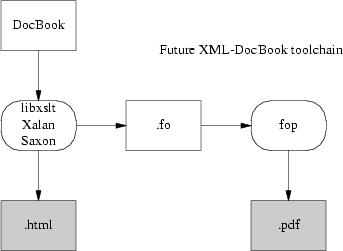
\includegraphics[]{figure3.png}}}

FOP has competition.  There is another project called
xsl-fo-proc\index{xsl-fo-proc}
which aims to do the same things as FOP, but in C++ (and therefore
both faster than Java and not relying on the Java environment).  As of
August 2002 FOP is in an unfinished alpha state, not as far along as
FOP.

% ------------------------   
% Section 
\section{Who are the projects and the players?}
\label{id2719568}\hypertarget{id2719568}{}%

The DocBook DTD itself is maintained by the DocBook Technical
Committee, headed by Norman Walsh.  Norm is the principal author of
the DocBook stylesheets, a man who has focused remarkable energy and
talent over many years on the extremely complex problems DocBook
addresses.  He is as universally respected in the DocBook/SGML/XML
community as Linus Torvalds is in the Linux world.

The \href{http://sources.redhat.com/docbook-tools/}{
docbook-tools} project provides open-source tools for
converting SGML DocBook to HTML, Postscript, and other formats.  This
package is shipped with Red Hat and other Linux distributions.  It is
maintained by Mark Galassi.

\href{http://www.jclark.com/jade/}{Jade} is an
engine used to apply DSSSL stylesheets to SGML documents.  It is
maintained by James Clark.

\href{http://openjade.sourceforge.net/}{OpenJade}
is a community project undertaken because the founders thought James
Clark's maintainance of Jade was spotty. The docbook-tools programs
use OpenJade.

\href{http://xmlsoft.org/XSLT/}{libxslt} is a C
library that interprets XSLT, applying stylesheets to XML documents.
It includes a wrapper program, {\bf xsltproc}, that can be
used as an XML formatter.  The code was written by Daniel Veillard
under the auspices of the GNOME project, but does not require any
GNOME code to run.  I hear it's blazingly fast compared to the 
Java alternatives, not a surprising claim.

\href{http://cyberelk.net/tim/xmlto/}{xmlto} is the
user interface of the XML toolchain that Red Hat ships.  It's written
and maintained by Tim Waugh.

\href{http://users.iclway.co.uk/mhkay/saxon/}{Saxon}
and \href{http://xml.apache.org/xalan-j/}{Xalan} are Java
programs that interpret XSLT.  Saxon seems to be designed to work
under Windows.  Xalan is part of the XML Apache project and native to
Linux and BSD; it's designed to work with FOP.

\href{http://users.ox.ac.uk/~rahtz/passivetex/}{PassiveTeX} the
package of LaTeX macros that xmlto uses for
producing DVI from XML-DocBook. \href{http://jadetex.sourceforge.net/}{JadeTex} is the package
of LaTeX macros that OpenJade uses for producing DVI from
SGML-DocBook.

\href{http://xml.apache.org/fop/}{FOP} translates
XML Formatting Objects to PDF.  It is part of the Apache XML project
and is designed to work with Xalan.

% ------------------------   
% Section 
\section{Migration tools}
\label{id2719718}\hypertarget{id2719718}{}%

The second biggest problem with DocBook is the effort needed to
convert old-style presentation markup to DocBook markup.  Human beings
can usually parse the presentatition of a document into logical
structure automatically, because (for example) they can tell from 
context when an italic font means `emphasis' and when it meabs
something else such as `this is a foreign phrase'.

Somehow, in converting documents to DocBook, those
sorts of distinctions need to be made explicit.  Sometimes
they're present in the old markup; often they are not, and the
missing  structural information has to be either deduced by 
clever heuristics or added by a human.

Here is a summary of the state of conversion tools from
various other formats:

\noindent
 
	\begin{description}
	\item[GNU Texinfo] 
The Free Software Foundation has made a policy decision to
support DocBook as an interchange format.  Texinfo has enough
structure to make reasonably good automatic conversion possible, and
the 4.x versions of {\bf makeinfo} feature a
{\tt{--docbook}} switch that generates DocBook.  More at the
\href{http://www.gnu.org/directory/texinfo.html}{makeinfo
project page}.
\item[POD] 
There is a \href{http://www.cpan.org/modules/by-module/Pod/}{POD::DocBook}
module that translates Plain Old Documentation markup to DocBook.  It
claims to support every DocBook tag except the L\textless{}\textgreater{} italic tag.
The man page also says "Nested =over/=back lists are not supported
within DocBook." but notes that the module has been heavily
tested.
\item[LaTeX] 
LaTeX is a (mostly) structural markup macro language built on
top of the TeX formatter.  There is a project called \href{http://www.lrz-muenchen.de/services/software/sonstiges/tex4ht/mn.html}{
TeX4ht} that (according to the author of PassiveTeX) can
generate DocBook from LaTeX.
\item[man pages and other troff-based markups] 
This is generally considered the biggest and nastiest conversion
problem.  And indeed, the basic
troff(1) markup is at too low a presentation
level for automatic conversion tools to do much of any good.  However,
the gloom in the picture lightens significantly if we consider
translation from sources of documents written in macro packages like
man(7).  These have enough structural
features for automatic translation to get some traction.

I wrote a tool to do this myself, because I couldn't find
anything else that did a half-decent job of it (and the problem is
interesting).  It's called \href{http://www.tuxedo.org/~esr/doclifter/}{doclifter}.  It will
translate to either SGML or XML DocBook from
man(7),
mdoc(7),
ms(7), or
me(7) macros.  See the documentation
for details.

	\end{description}
    
% ------------------------   
% Section 
\section{Editing tools}
\label{id2719956}\hypertarget{id2719956}{}%

One thing we presently do not have is a good open-source
structure editor for SGML/XML documents.

\href{http://www.lyx.org/}{LyX} is a GUI word processor
that uses LaTeX for printing and supports structural editing of LaTeX
markup.  There is a LaTeX package that generates DocBook, and a
\href{http://bgu.chez.tiscali.fr/doc/db4lyx/}{how-to document}
escribing how to write SGML and XML in the LyX GUI.

\href{http://idx-getox.idealx.org/}{GeTox}, the
GNOME XML Editor, aims at nontechnical users.  But the software is
still (as of August 2001) alpha, more a proof of concept than anything
useful, and the project group seems not to be very active; there have
been no updates of the website between May 2001 and August 2002 (time of
writing).

\href{http://www.math.u-psud.fr/~anh/TeXmacs/TeXmacs.html}{ GNU
TeXMacs} is a project aimed at producing an editor that is good
for technical and mathematical material, including displayed formulas.
1.0 was released in April 2002.  The developers plan XML support in
the future, but it's not there yet.

\href{http://www.freesoftware.fsf.org/thotbook/}{ThotBook}
is a project to put together a GUI editor for DocBook based on
the Thot toolkit.  It way be moribund; the web page was not updated
from November 2001 to August 2002 (time of writing).

Most people still hack the tags by hand using either vi or Emacs, using
psgml to validate the results.

% ------------------------   
% Section 
\section{Related standards and practices}
\label{id2717112}\hypertarget{id2717112}{}%

The tools are coming together, if slowly, to edit and format
DocBook markup. But DocBook itself is a means, not an end.  We'll need
other standards besides DocBook itself to accomplish the
searchable-documentation-database objective I laid out at the
beginning of this document. There are two big issues: document
cataloguing and metadata.

The \href{http://scrollkeeper.sourceforge.net/}{Scrollkeeper}
project aims directly to meet this need. It provides a simple set of
script hooks that can be used by package install and uninstall
productions to register and unregister their documentation.

Scrollkeeper uses the \href{http://www.ibiblio.org/osrt/omf/}{ Open Metadata Format}.
This is a standard for indexing open-source documentation analogous to
a library card-catalog system.  The idea is to support rich search
facilities that use the card-catalog metadata as well as the source 
text of the documentation itself.

% ------------------------   
% Section 
\section{SGML and SGML-Tools}
\label{id2717159}\hypertarget{id2717159}{}%

In previous sections, I have thrown away a lot of DocBook's
history.  XML has an older brother,
SGML\index{SGML} or Standard Generalized
Markup Language.

Until mid-2002, no discussion of DocBook would have been
complete without a long excursion into SGML, the differences between
SGML and XML, and detailed descriptions of the SGML DocBook toolchain.
Life can be simpler now; a XML DocBook toolchain is available in open
source, works as well as the SGML toolchain ever did, and is easier to
use, If you don't think you'll ever have to deal with old SGML-Docbook
documents, you can skip the remainder of this section.
\subsection{DocBook SGML}
\label{id2717193}\hypertarget{id2717193}{}%

DocBook was originally an SGML application, and there was an
SGML-based DocBook toolchain that is now moribund.  There are minor
differences between the DocBook SGML DTD and the DocBook XML DTD, but
for an introductory discussion we can ignore them. The only one that's
normally user-visible is that in SGML contentless tags did not need to
have a trailing slash added to them before the closing \textgreater{}.
(Requiring the trailing / means XML parsers can be a lot simpler,
because they don't have to know about the DTD to know which opening
tags need closers.)

Versions of HTML up to 4.01 (before XHTML) were SGML
applications.  TEI was originally an SGML application, too.  The
groups managing all three DTDs jumped to XML for the same reason
DocBook's developers did --- it's drastically simpler.  SGML was
extremely complex; unmanageably so, as it turns out.  The
specification was a dense 150 pages and it is not reliably reported
that any software ever fully implemented it.

The toolchain diagram I gave earlier was simplified; it
only showed the XML toolchain.  Here is the historically
correct version:
{{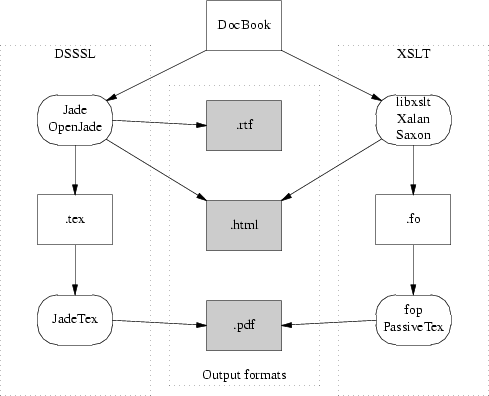
\includegraphics[]{figure4.png}}}

The DSSSL toolchain is what processed DocBook SGML.
Under it, a document goes from DocBook format through one of two
closely-related stylesheet engines called Jade and OpenJade.  These
turn it into a TeX-macro markup. which is processed by a package called
JadeTeX, into DVIs, which then get turned into Postscript.
\subsection{Why SGML DocBook is dead}
\label{id2717259}\hypertarget{id2717259}{}%

The DSSSL toolchain is, as far as new development goes,
effectively dead.  The XSLT toolchain has just reached production
status as I write in August 2002; a working version shipped in Red Hat
7.3.  It's where DocBook developers are putting almost all of their
effort.

The reason for the change to XML was threefold.  First,
SGML turned out to be too complicated to use; then, DSSSL turned out
to be too complicated to live with; then, significant parts of the
DSSSL toolchain turned out to be weak and irredeemably messy.

Relative to SGML, XML has a reduced feature set that is
sufficient for almost all purposes but much easier to understand and
build parsers for.  SGML-processing tools (such as validating parsers) have
to carry around support for a lot of features that DocBook and other
text markup systems never actually used.  Removing these features
made XML simpler and XML-processing tools faster.

The language used to describe SGML DTDs is sufficiently spiky
and forbidding that composing SGML DTDs was something of a black art.
XML DTDs, on the other hand, can be described in a dialect of XML
itself; there does not need to be a separate DTD language. An XML
description of an XML DTD is called a
{\em schema}\index{schema};
the term DTD itself will probably pass out of use as the standards for
schemas firm up.

But mostly the DSSSL toolchain is dead because DSSSL itself, the
SGML stylesheet description language in that toolchain, proved just too
arcane for most human beings, and made stylesheets too difficult to
write and modify. (It was a dialect of Scheme.  Your humble editor, a
LISP-head from way back, shakes his head in sad bemusement that
this should drive people away.)

XML fans like to sum up all these changes with "XML: tastes great, less
filling."
\subsection{SGML-Tools}
\label{id2717333}\hypertarget{id2717333}{}%

SGML-Tools was the name of a DTD used by the \href{http://www.linuxdoc.org}{Linux Documentation Project},
developed a few years ago when today's DocBook toolchains didn't exist.
SGML-Tools markup was simpler, but also much less flexible than
DocBook.  The original SGML-Tools formatter/DTD/stylesheet(s)
toolchain has been dead for some time now, but a successor called \href{http://sourceforge.net/projects/sgmltools-lite/}{SGML-tools
Lite} is still maintained.

The LDP has been phasing out SGML-Tools in favor of DocBook, but
it is still possible you might take over an old HOWTO.  These can be
regognized by the identifying header "\textless{}!doctype linuxdoc
system\textgreater{}. If this happens to you, convert the thing to XML DocBook
and give the old version a quick burial.

% ------------------------   
% Section 
\section{References}
\label{id2717368}\hypertarget{id2717368}{}%

One of the things that makes learning DocBook difficult is that
the sites related to it tend to overwhelm the newbie with long lists
of W3C standards, massive exercises in SGML theology, and dense
thickets of abstract terminology.  We're going to try to avoid that
here by giving you just a few selected references to look at.

Michael Smith's \href{http://xml.oreilly.com/news/dontlearn_0701.html}{
Take My Advice: Don't Learn XML} surveys the XML world from
an angle similar to this document.

Norman Walsh's {\em DocBook: The Definitive
Guide} is available \href{http://www.oreilly.com/catalog/docbook/}{in print} and
\href{http://www.docbook.org/tdg/en/html/docbook.html}{on the
web}.  This is indeed the definitive reference, but as an
introduction or tutorial it's a disaster.  Instead, read this:

\href{http://www.bureau-cornavin.com/opensource/crash-course/index.html}{Writing 
Documentation Using DocBook: A Crash Course}.  This is an excellent
tutorial.

There is an excellent \href{http://www.dpawson.co.uk/docbook/}{DocBook FAQ} with a lot
of material on styling HTML output.  There is also a DocBook \href{http://docbook.org/wiki/moin.cgi}{wiki}.

If you're writing for the Linux Documentation Project, read the
\href{http://www.linuxdoc.org/LDP/LDP-Author-Guide/index.html}{
LDP Author Guide}.

The best general introduction to SGML and XML that I've
personally read all the way through is David Megginson's \href{http://vig.pearsoned.com/store/product/0,,store-562_banner-0_isbn-0136422993,00.html}{Structuring
XML Documents} (Prentice-Hall, ISBN: 0-13-642299-3).

For XML only, \href{http://www.oreilly.com/catalog/xmlnut2/}{XML In A Nutshell}
by W. Scott Means and Elliotte "Rusty" Harold is very good.

\href{http://www.ibiblio.org/xml/books/bible/}{The XML
Bible} looks like a pretty comprehensive reference on XML and
related standards (including Formatting Objects).

Finally, the \href{http://xml.coverpages.org/}{The XML
Cover Pages} will take you into the jungle of XML standards
if you really want to go there.

% --------------------------------------------
% End of document
% --------------------------------------------
\end{document}
